\section{C-gen}
\label{sec:cgen}
A ferramenta C-gen foi desenvolvida como trabalho de conclusão de curso (TCC) por Jerônimo Backes, pela Universidade de Santa Cruz do Sul (UNISC) em 2005. O propósito da ferramenta é de auxiliar o estudo das três fases de construção de um compilador, sendo elas a análise léxica, análise sintática e análise semântica. Segundo \cite{cgen}, no curso de compiladores é comum a implementação de um pequeno compilador, ou partes deles, para aplicar o conhecimento teórico aprendido em sala de aula. Porém, em cada fase, podem ser aplicados diversos métodos bastante complexos, o que dificulta o aprendizado do aluno. 

Existem ferramentas que auxiliam na construção de um compilador, mas a maioria delas são usadas em apenas uma fase do compilador e são destinadas ao uso profissional \cite{cgen}, sendo assim ferramentas nada didáticas e de fácil uso.  

A ferramenta C-gen foi desenvolvida após a análise de características de três ferramentas profissionais, \textit{Flex}\footnote{http://flex.sourceforge.net/}, \textit{Bison}\footnote{http://www.gnu.org/software/bison/} e \textit{COCO/R}\footnote{http://www.ssw.uni-linz.ac.at/coco/}, levando em conta seus pontos positivos e negativos sobre a ótica educacional. 

\begin{figure}[ht!]
	\centering
	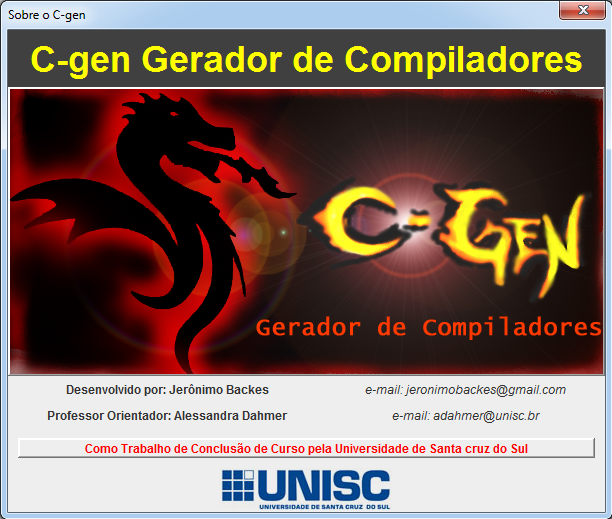
\includegraphics[scale=0.7]{imgs/cgen.png}
	\caption{A ferramenta C-gen.}
	\label{cgen-inicial}
\end{figure}

\newpage
C-gen possui interface gráfica bastante fácil e intuitiva, não sendo necessário programar a entrada como em outras ferramentas, o que sem dúvidas facilita a interatividade com o aluno, e portanto, o aprendizado. Apesar da ferramenta realizar as fases de análise léxica, análise sintática e análise semântica, o escopo desse trabalho se limitou apenas na fase de análise léxica.

\begin{figure}[ht!]
	\centering
	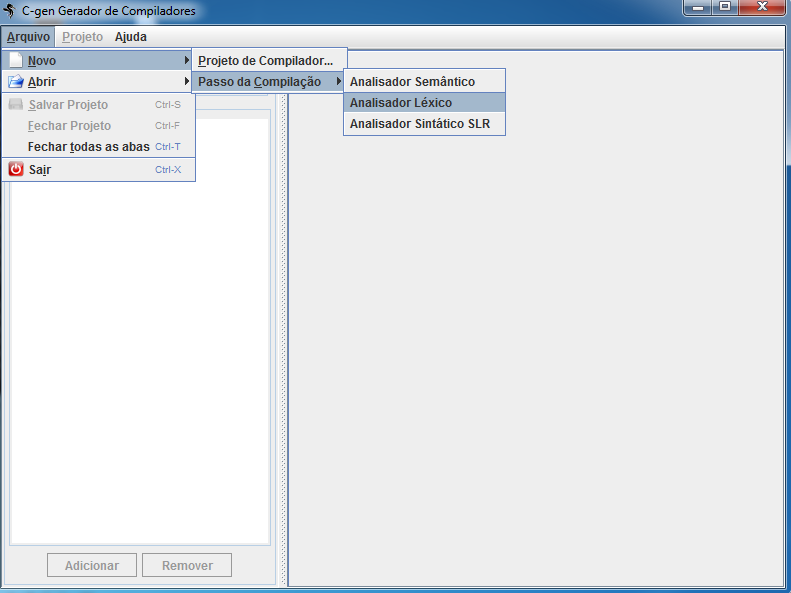
\includegraphics[scale=0.5]{imgs/cgen2.png}
	\caption{Criando um projeto para a análise léxica.}
	\label{cgen-analise-lexica}
\end{figure}

Após criar um projeto para a fase de análise léxica, a ferramenta abre um editor de autômatos como mostra a figura \ref{cgen-automatos}, que será utilizado para o reconhecimento dos \textit{tokens}. O editor é de fácil uso e nele é configurado os estados, as transições entre eles, qual é o estado inicial, quais são os estados finais e quais são os \textit{tokens} reconhecidos por cada estado final. Nas transições dos estados, é possível escolher quais caracteres serão consumidos, onde ``>>'' representa ``o que estiver entre''.

\begin{figure}[ht!]
	\centering
	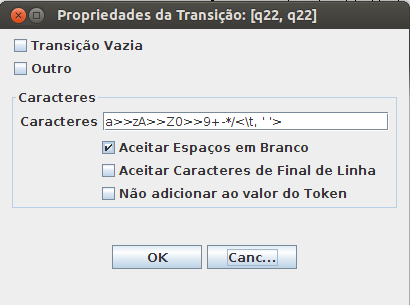
\includegraphics[scale=0.59]{imgs/cgen5.png}
	\caption{Exemplo de transição que consome qualquer caractere de a até z, A até Z, 0 até 9 entre outros.}
	\label{cgen-transicoes}
\end{figure}

\begin{figure}[ht!]
	\centering
	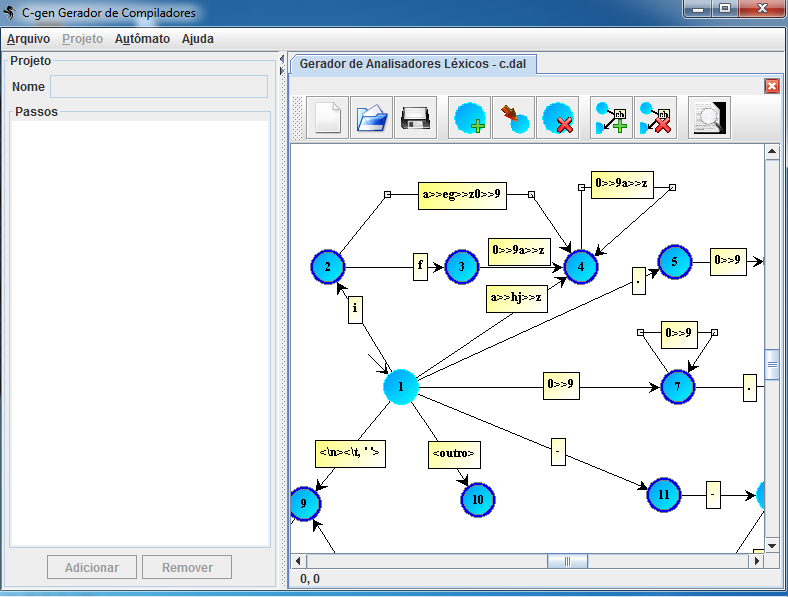
\includegraphics[scale=0.55]{imgs/cgen3.png}
	\caption{Editor de autômatos da ferramenta C-gen.}
	\label{cgen-automatos}
\end{figure}

A ferramenta também possui opções para inserir as palavras reservadas da linguagem como mostra a figura \ref{cgen-reservadas}.

\begin{figure}[ht!]
	\centering
	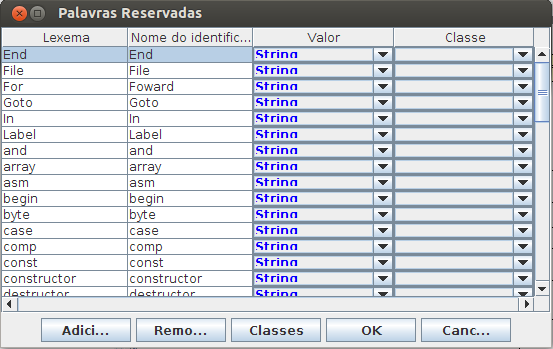
\includegraphics[scale=0.7]{imgs/cgen6.png}
	\caption{Inclusão de palavras reservadas.}
	\label{cgen-reservadas}
\end{figure}

Ao término de toda configuração, é executado a análise léxica para o reconhecimento dos \textit{tokens}. Nessa parte, é possível visualizar a matriz de transição dos estados como mostra a figura \ref{cgen-matriz}. Nesse momento, a ferramenta possui diversas opções como executar a análise  caractere a caractere, ou por \textit{tolken} e até por um intervalo de tempo predeterminado.

\newpage
\begin{figure}[ht!]
	\centering
	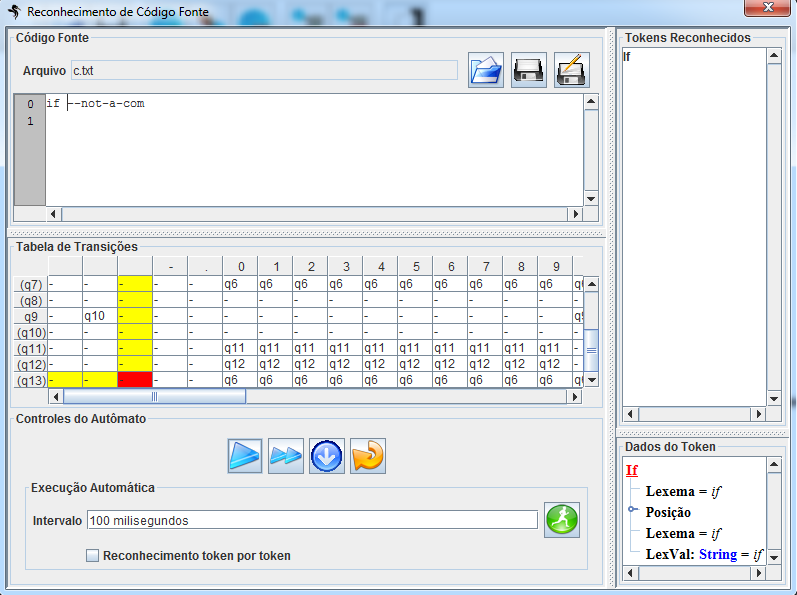
\includegraphics[scale=0.5]{imgs/cgen4.png}
	\caption{Matriz de transições.}
	\label{cgen-matriz}
\end{figure}

\subsection{Considerações}
\label{sub:cgen-consideracoes}

\begin{table}[ht]
\caption{Considerações de algumas características das ferramentas}
\centering
\begin{tabular}{|m{1.6cm}|m{1.5cm}|m{1.5cm}|m{1.5cm}|m{1.5cm}|m{1.8cm}|m{1.5cm}|}  \hline
   Ferramenta & Design da interface com o usuário & Facilidade de uso da ferramenta & Interação com o usuário & Facilidade de aplicação da fundamentação teórica & Capacidade de aplicação das ramificações teóricas & Relação entre uso e aprendizado \\ \hline
C-gen & Bom & Bom & Bom & Bom & -- & Bom \\ \hline
\end{tabular}
\label{table:caracteristicas}
\end{table}


A ferramenta C-gen, na parte de análise léxica (o escopo desse trabalho) é uma ferramenta de fácil uso, onde não é necessário programar a entrada, pois possui um editor de autômato junto a ferramenta. Sua interface gráfica é intuitiva e amigável ao usuário e possui diversas opções para visualizar o reconhecimento dos \textit{tokens}, mostrando passo a passo o que está acontecendo na análise. A ferramenta porém, possui um ponto negativo ao entrar no processo de reconhecimento. O autômato de entrada é convertido para um autômato finito determinístico, onde os identificadores dos estados no autômato mudam após a conversão apenas na matriz de transição. Isso, dificulta acompanhar o reconhecimento pela matriz de transições junto ao autômato. Além disso, caso a conversão seja executada mesmo que o autômato já seja determinístico, o autômato resultante da conversão pode apresentar configursações inúteis. A ferramenta possui fácil aplicação da fundamentação teórica uma vez que possui opções para a análise léxica, sintática e semântica. Como a parte de análise léxica não possui diversas abordagens (como por exemplo, na análise sintática, abordagens \textit{bottom-up} e \textit{top-down}), sobre o aspecto da capacidade de aplicação das ramificações teóricas não se pode dar um julgamento. Por fim, a ferramenta C-gen possui um manual que explica qual a função de cada passo do compilador, com exemplos de como utilizar a ferramenta, o que mesmo para um aluno que não domina o conteúdo teórico em sua totalidade, ainda assim pode utilizar a ferramenta com certa facilidade.




